\documentclass[border=5mm]{standalone}
\usepackage{pgfplots}
\usepackage{tikz}
\pgfplotsset{compat=1.8}
\pgfdeclarefunctionalshading{sphere}{\pgfpoint{-25bp}{-25bp}}{\pgfpoint{25bp}{25bp}}{}{
%% calculate unit coordinates
25 div exch
25 div exch
%% copy stack
2 copy 
%% compute -z^2 of the current position 
dup mul exch
dup mul add
1.0 sub
%% and the -z^2 of the light source 
0.3 dup mul
-0.5 dup mul add
1.0 sub
%% now their sqrt product
mul abs sqrt
%% and the sum product of the rest
exch 0.3 mul add
exch -0.5 mul add
%% max(dotprod,0)
dup abs add 2.0 div 
%% matte-ify
0.6 mul 0.4 add
%% currently there is just one number in the stack.
%% we need three corresponding to the RGB values
dup
0.4
}
\begin{document}
      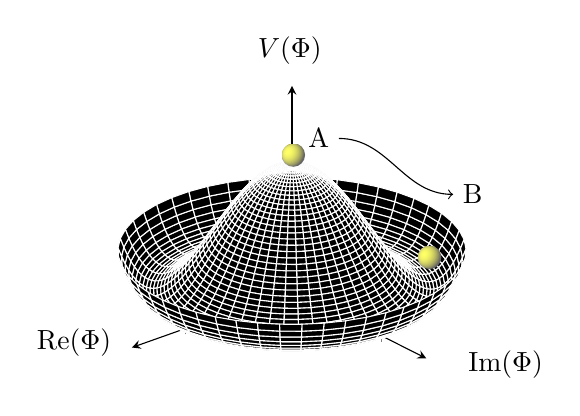
\begin{tikzpicture}
          \begin{axis}[  axis lines=center, axis on top = false, 
           view={140}{25},axis equal,title={},
          colormap={blackwhite}{gray(0cm)=(1); gray(1cm)=(0)},
            samples=50,
            domain=0:360,
            y domain=0:1.25,
            zmin=0,
        xmax=1.5,
        ymax=1.5,
        zmax=1.5,
        x label style={at={(axis description cs:0.10,0.25)},anchor=north},
        y label style={at={(axis description cs:0.9,0.2)},anchor=north},
        z label style={at={(axis description cs:0.5,0.9)},anchor=north},
        xlabel = $\mathrm{Re}(\Phi)$,
        ylabel=$\mathrm{Im}(\Phi)$,
        zlabel=$V(\Phi)$,
        yticklabels={,,},
        xticklabels={,,},
        zticklabels={,,}
        ]
        \addplot3 [surf, shader=flat, draw=white, fill=black, z buffer=sort] ({sin(x)*y}, {cos(x)*y}, {(y^2-1)^2});
        \end{axis}
        \shade[shading=sphere] (3.47,3.5) circle [radius=0.15cm];
        \shade[shading=sphere] (5.2,2.2) circle [radius=0.15cm]; 
        \node[anchor=east] at (4.05,3.71) (text) {A};
  \node[anchor=west] at (5.5,3.0) (description) {B};
  \draw (description) edge[out=180,in=0,<-] (text);
    \end{tikzpicture}
\end{document}